\chapter{メールアカウントデータベース構造の設計}

LDAPで、データベースをデザインするということは、ツリー構造をデザインするということです。
メールアカウント情報の外部データベースとしてLDAPを使用する場合、どのようなデザインにすればよいか、本章ではそれについて説明をします。

\section{アカウントデータベースの大まかな形}

\begin{figure}[htbp]
	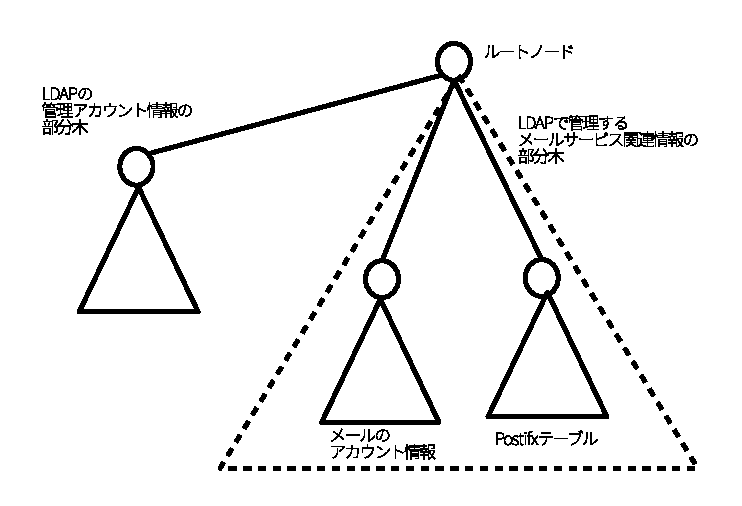
\includegraphics[width=12cm,clip]{draw/abstruct.eps}
	\caption{メールのアカウントデータベースの概要}
	\label{fig:abstruct}
\end{figure}

メールアカウントとして使うLDAPツリーを構成するとき、どのようなツリー構造にすれば良いのでしょうか。
慣例的に、LDAPツリーのルートノード以下は、LDAPそのものの管理アカウント情報を入れる部分木と、LDAPで管理したい情報を入れる部分木から構成されます。
今回、LDAPで管理したい情報はメールに関するアカウント情報です。

また、aliases(5)など、左辺と右辺がい一対一であるPostfixテーブルで管理するデータはLDAPで管理することが可能です。
ただし、Postfixテーブルで左辺にワイルドカードを伴うなど、右辺と左辺が一対一でないテーブルは、LDAPに入れることはできません。その場合は、取りうる値を展開して、一つ一つのノードにする必要があります。
この点は注意をしてください。

LDAPで管理したい情報の中で、メールアカウントに関する部分木と、Postfixテーブルに関する部分木を分割します。これが、今回構築するメールアカウントデータベースの大まかな形です。

\subsection{ルート部分}

\begin{figure}[htbp]
	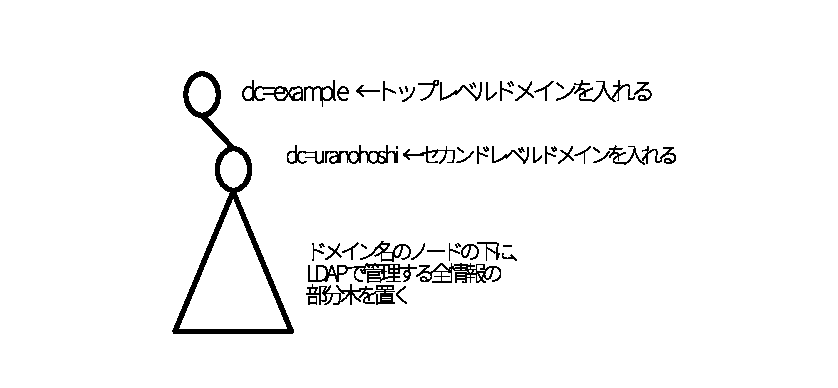
\includegraphics[width=12cm,clip]{draw/dc.eps}
	\caption{Domain Context}
	\label{fig:dc}
\end{figure}

図\ref{fig:dc}のように、ルート部分は、慣例として、メールアドレスを管理するドメインのTLDをDNとします。たとえば、uranohoshi.exampleであれば、DN:dc=exampleというようにします。dcは、domain contextという属性です。慣例的に、この下にdcでセカンドレベル以降のドメインをつなげます。これは、dcという属性の標準的な使い方です。

複数のドメインに着いて管理したい場合は、ルートをたとえば、dc:rootというようにルートであるように記述して、その子ノードとして、dc=uranohoshi.exampleと、dc=otonoki.exampleを置き、それを起点とする部分木をそれぞれのドメインのデータベースにする、という方法もあります。

ですが、コンテナなどでPaaSインスタンスを調達しやすい現在では、ドメイン毎に独立したLDAPインスタンスを用意する方がよいという考えもあります。この方法を採る場合、ACLの構成をシンプルにできるというメリットがあります。欠点は、ドメイン毎にLDAPサーバがひとつ立ち上がっている状態になる、とういうことですが、リソース調達の容易な現代では問題にならないでしょう。

\subsection{ドメイン名以下の子ノード}

\begin{figure}[htbp]
	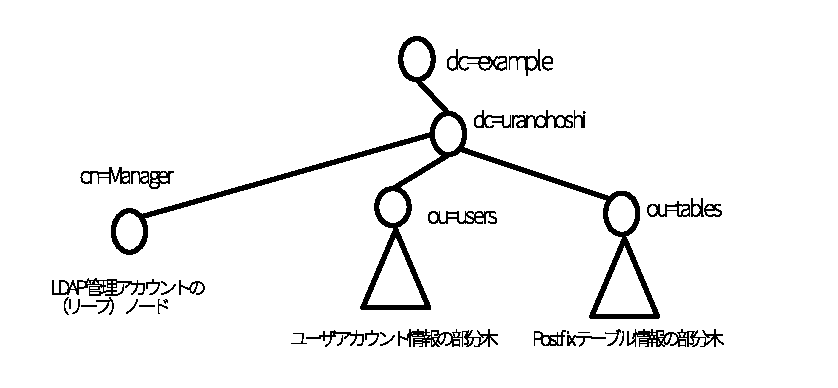
\includegraphics[width=12cm,clip]{draw/structure.eps}
	\caption{dc以下の木構造}
	\label{fig:structure}
\end{figure}

ルートノード以下は、管理アカウント、ユーザアカウント、エイリアスなどPostfixテーブルのサブツリーに分けます。ここでは、ユーザアカウントと、Postfixテーブル部分について解説します。

それぞれのRDNをあらわすのに使う属性は、オブジェクトタイプtopに含まれる属性のouを使います。本来は、Organization Unitで、組織内の部門を著わすのに使う属性値ですが、LDAPツリーの部分木の起点である子とを著わすために、便宜的に使用されます。

ここでは、ou=usersとou=tablesというRDNをもつ二つのノードを作ることにしましょう。これらのノードは、それぞれユーザアカウント情報とPostfixテーブル情報の部分木の基点となります。
また、cn=Managerとして、LDAPの管理に使うアカウント情報を格納します。

\subsection{管理アカウントのノード}

LDAPそのものの管理アカウント情報は、LDAOPの木の中に含めます。慣例として、ドメイン名のノードの直下に、管理アカウント情報のノードを置きます。この場所は、LDAPサーバの設定で指定します。OpenLDAPの場合は、slapd.conf(5)の中で、以下のように設定します。

\begin{verbatim}
rootdn "cn=Manager,dc=uranohoshi,dc=example"
rootpw password
\end{verbatim}

パスワードは設定ファイルに記述してあるので、dn:cn=Manager,dc=uranohoshi,dc=exampleの中には記述しません。

\section{ユーザアカウント情報}

ユーザアカウント情報の部分木は、ユーザ情報とメールアドレスの関係を参照するのに使う部分木です。この部分は、ひとつひとつのユーザアカウントに対応するノードで構成されます。この部分木をどう作るか、ノードにどんな除法を含めるかについて、説明します。

\subsection{ユーザアカウントの部分木の構造}

\begin{figure}[htbp]
	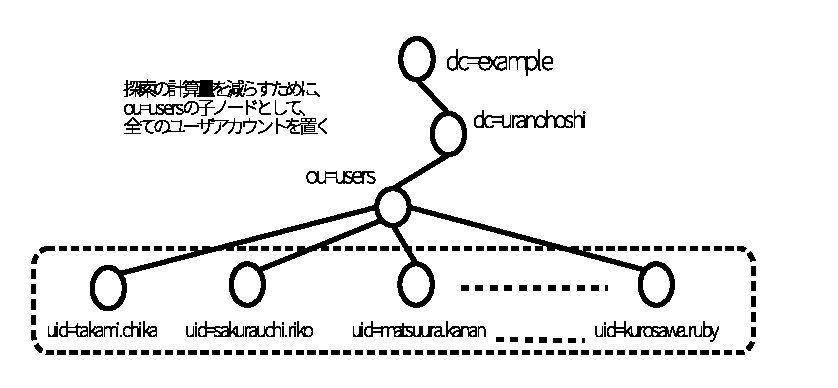
\includegraphics[width=12cm,clip]{draw/users.eps}
	\caption{ユーザアカウントの部分木}
	\label{fig:users}
\end{figure}

ユーザアカウント情報は、ou=usersのノード以下に、全てのメールアカウントがある構造にします。こうすることで、ユーザアカウントに関する検索を、高速化することができます。
ユーザのグループ分けが必要な場合は、ユーザアカウントのノードにgroup属性やgid属性を置き、その値でグループ分けを行うようにします。

ou=usersのしたに、ユーザグループとしての部分木の起点として、ou=部署(グループ)名とのノードを置き、その子ノードとして、部署に所属するユーザからなる部分木を作るやり方もあります。ですが、この方法は、グループ単位でユーザ管理のACLを設定したい場合でないなら、推奨しません。

これは、ユーザやメールアドレスをキーに検索するときに、条件としてグループが判明していない場合が多々あります。この場合、部分木の再帰検索となるため、時間が多くかかります。
また、人事など、アナログな組織に対応してグループ分けをした場合など、そのユーザアカウントに対応するユーザの異動などで、別のグループに移ったとき、そのアカウントをDITの別の部分に移さなければならなくなり、管理の工数が増加します。

\subsection{ユーザアカウントのノード}

ユーザアカウントに関するノードは、どのような情報を入れれば良いのでしょうか。基本的に、オブジェクトタイプinetOrgPersonをもとにしておけば多くの場合用が足ります。
inetOrgPersonは、認証を伴うユーザアカウントを定義するオブジェクトタイプです。DNには、ユーザIDである属性uidを使います。

例えば、dn:dc=example,dc=uranohoshi,ou=users以下のノードに、matsuura.kanan@uranohoshi.exampleのユーザアカウント情報を置くとして考えてみましょう。このノードは、inetOrgPersonとorganizationalPersonと、posixAccountという三つのオブジェクトタイプを使って、以下のLDIFのようにあらわされます。

\begin{verbatim}
dn: uid=matsuura.kanan,ou=users,d=uranohoshidc=example
changetype: add
objectclass: inetOrgPerson
objectClass: posixAccount
uid: matsuura.kanan
gid: AZELIA
userPassword: xxxxxxx
uidNumber: 1001
gidNumber: 100
mail: matsuura.kanan@uranohosi.example
cn: 松浦果南
homeDirectory: /home/matsuura.kanan
description: 淡島に住んでいる
\end{verbatim}

ここで新しく出てきた属性を、簡単に説明します。

\paragraph{uid}
ユーザIDです。メールアドrスト一致させるのが一般的ですが、メールアドレスとことなるuidを使うこともできます。

\paragraph{gid}
グループidです。UNIXなどのOSでの、グループ名に相当する属性になります。

\paragraph{userPassword}
このユーザアカウントで認証をするときに用いる、パスワード文字列です。この例では暗号化されていないプレーンテキストですが、暗号化したもの、ハッシュ値を記載することもできます。

\paragraph{uidNumber}
ユーザIDの番号です。UNIXなどのOSで、uidに紐付いている数字になります。

\paragraph{gidNumber}
グループIDの番号です。これも、UNIXなどのOSで、gid二紐付いている数字になります。

\paragraph{mail}
メールアドレスです。このユーザアカウントに対応しているメールアドレスになります。ひとつのユーザアカウントに複数対応させることもあります。

\paragraph{cn}
common nameの略です。ユーザアカウントに対応するユーザの本名を格納する場合などに使います。UTF-8のマルチバイトの場合は、実際にはBASE64エンコードして格納します。

\paragraph{homeDirectory}
ユーザアカウントに対応するホームディレクトリの絶対パスを格納します。PostfixをMaildir/形式で使用する場合、このディレクトリ以下に、ディレクトリのMaildir/が置かれます。

\paragraph{description}
そのノードの注釈をテキストで書くための属性です。記述内容がUTF-8のマルチバイトであった場合は、実際にはBASE64エンコードでデータが格納されます。

\subsection{実ユーザとバーチャルユーザ}

LDAPでユーザアカウント情報を管理する場合、メールサーバの実ユーザにするか、メールアカウントだけのバーチャルユーザにするかという選択肢があります。
実ユーザは、LDAPのユーザアカウント情報が、メールサーバにログイン可能なユーザアカウント情報となるように設定することです。メールアカウントの一部に、メールサーバへのシェルログインを許したい場合、実ユーザとして設定してやる必要があります。このときは、ホストのPAMで、ユーザアカウントのノードを参照するように設定します。

実ユーザにしたときの利点は、ホストのユーザアカウントを設定できるツールで、パスワードの設定が可能であることです。そのため、既存のプロダクトを導入して、パスワード変更サービスなどを導入することができます。また、メールデータを置くホームディレクトリのアクセス制御や、容量制限の制御(クオータ)に、OSの支援を受けられるというメリットもあります。
またPostfixの標準設定では、OSのユーザ情報を、そのままメールアドレスとして使用し、ユーザのホームディレクトリにメールデータを置くようになっています。

ですが、これは逆にいうと、ユーザ数の上限など、OSの影響を受けると言うことにもなります。また、サーバそのものがLDAPに置かれているユーザ情報の影響を受けるため、セキュリティ的に弱いということもデメリットです。
その例として、PostfixをMaildir/形式で運用する場合、Postfixはユーザのホームディレクトリにアクセス可能な権限で動かす必要があります。

さらに、ユーザアカウントが特定のサーバに紐付くことから、クラスタリングが行いにくくなる、というデメリットもあります。


バーチャルユーザは、Postfixのメールアカウントと、それに対応する認証のみを行なうためのデータベースとして、ユーザアカウント情報を使用する方法です。メリット、デメリットは、実ユーザと逆になります。
バーチャルユーザは特定のホストに紐付きません。そのため、ユーザアカウントデータベースを抽象化することでクラスタリングが行いやすくなります。また、メールデータを置くホームディレクトリのアクセス権のオーナシップを、Postfixが管理する運用にすることもできます。

その半面、設定が複雑化したり、OSの支援が受けられない、という欠点も生じます。メールアドレス毎に、メールを格納する場所も、定義する必要があります。

そのため、ある程度ユーザ規模が大きい場合や、MTAとMRAを分けて運用する場合など、デメリットを許容できる場合でないと、バーチャルユーザは使いにくくなります。


\section{Postfixテーブル情報}

\begin{figure}[htbp]
	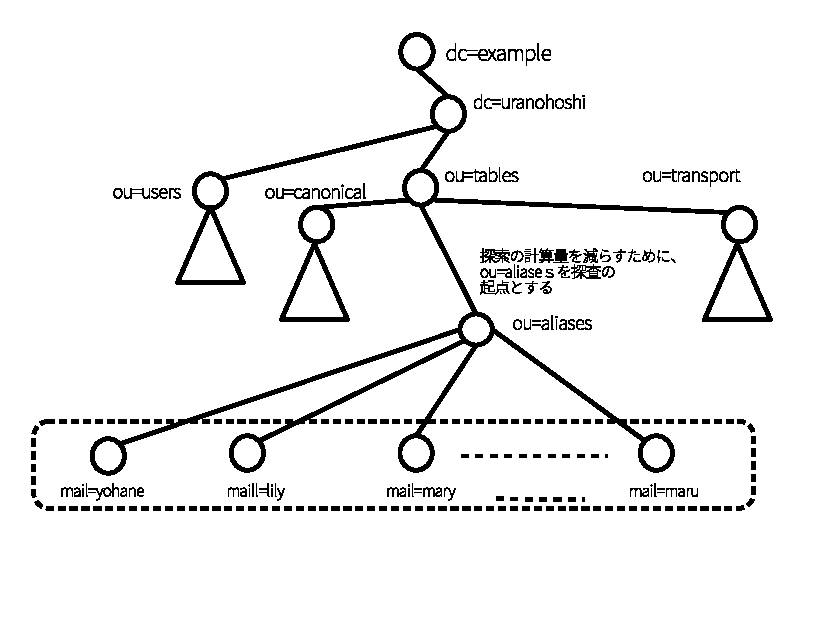
\includegraphics[width=12cm,clip]{draw/postfix_table.eps}
	\caption{Postfixテーブルの部分木}
	\label{fig:postfix_table}
\end{figure}

Postfixテーブルで、左辺がひとつに定まるものは、LDAPのノードに入れることができます。これは、左辺がワイルドカードや正規表現などで、複数の値がマッチングするものは、LDAPには入れられないということです。ただし、左辺で取りうる値を全て網羅し、一つ一つの子ノードに展開してやることで、そのPsotfixテーブルをLDAPに収容することが可能です。

わかりやすくするため、図\ref{fig:postfix_table}のように、ou=tablesの子ノードとして、ou=aliases、ou=canonical、ou=transport、というように、どのテーブルに対応する部分木かがわかるようにノードを追加します。


\subsection{エイリアステーブル}

例として、左辺がひとつに定まるものとして、エイリアステーブルを考えてみましょう。エイリアステーブルは、左辺がひとつのメールアドレス、右辺が一つ以上のメールアドレスになります。
以下のような、alias(8)の、sendmail互換形式のエイリアステーブルを、LDAPのノードとして組み込むための、LDIFにしてみましょう。

\begin{verbatim}
# lily@uranohoshi.exampleのエイリアステーブル
lily:  sakurauchi.riko@uranohosi.example , 
       sakurauchi@otonoki.example
\end{verbatim}

この子ノードは、DNとして、mail=likyを取るようにします。また、転送先を洗わず属性を一つ以上持つことができるオブジェクトタイプ、postfixTableAliasがあるとして定義しましょう。
また、maildropという属性値は、postfixTableAliasで定義されていることにします。
このエイリアスのノードは、DN:dc=example,dc=uranohoshi,ou=tables,ou=aliases,mail=lilyとなります。

\begin{verbatim}
dn: mail=lily,ou=aliases,ou=tables,dc=uranohoshi,dc=example
changetype: add
objectclass: top
objectclass: postfixTableAlias
mail: lily
maildrop: sakurauchi.riko@uranohoshi.example
maildrop: sakurauchi@otonoki.example
mailEnable: OK
\end{verbatim}

\subsection{Postfixテーブルの属性}

Postfixテーブルは、LDAP規定のオブジェクタイプで、そのまま使え沙ものは多くありません。先程のエイリアステーブルのノードも、スキーマファイルで属性を定義した前提で提示しています。

これは、LDAPの標準的な属性として、メールのエイリアスを記述するためのものが含まれていないためです。LDAPでは、環境やアプリケーションに依存しない属性を、標準的なものとして、オブジェクトタイプとして定義しています。

この、Postfixテーブル形式の、エイリアステーブルのように、特定の実装で必要になる属性は、スキーマファイルで定義する必要があります。

\subsection{どこから探査するか}

ユーザアカウントの場合、ou=usersのすぐ下に、ユーザアカウントのノードを置くべき、という説明をしました。ですが、Postfixテーブルでは、ou=tablesnの下に、何のテーブルかを著わすouのノードを置き、その下にテーブルの内容を子ノードとして置く、という説明です。
なぜ、ユーザアカウントとPostfixテーブルは、このように違うのでしょうか。

Postfixテーブルを検索するときは、どのテーブルに対応する兄弟ノードを参照するかを決め打ちすることができます。例えば、エイリアスの情報を見たいときに、カノニカルの情報が入れられている部分木を見る必要はありません。そのため、本書の例であれば、dn:ou=aliases,ou=tables,dc=uranohoshi,dc=exampleノードを親とする兄弟ノードのみを、探索の範囲とすれば良いということになります。

一方、ユーザアカウントで、ou=usersの下に、ユーザの所属を著わすouを置いておいた場合を考えましょう。ユーザアカウント参照時に、ユーザの所属するouがどれか、決め打ちができません。そのため、再帰探索が生じるため、本書では、このような構成はおすすめできない、ということにしています。

\section{属性の追加}

エイリアステーブルのところで説明に使用した、maildropという属性は、オブジェクトタイプinetOrgPersonにはありません。
これは、新しいオブジェクトタイプとして定義したものです。ここでは、スキーマの追加の必要性と、追加方法について説明します。

\subsection{属性追加の必要性}

ISO/ITU-Tによって定義されていない属性を使うときは、スキーマで属性を追加する必要があります。これは、既存の属性では、属性名や属性そのものが足りない場合など、属性を追加します。

たとえば、ホームディレクトリのクオータは、標準の属性にはありません。そのため、ユーザアカウントのノードに情報を持たせるには、属性を追加する必要があります。

また、たとえばmailEnableという属性を作ったとしましょう。検索したい値と、mailEnableの値をAND検索することで、そのノードの情報が有効か無効化のスイッチに使うことができます。


\subsection{スキーマファイルによる追加}

属性と、それをまとめたオブジェクトタイプは、スキーマファイルというテキストの設定ファイルによって、追加する事ができます。OpenLDAPの場合は、そのDITで使用するスキーマはslapd.conf(5)に記述します。

OpenLDAPのソースツリーには、拡張子.schemaで基本的なスキーマファイルが付属しています。また、独自のスキーマファイルを策せ強いた場合も、同様に追加する事ができます。このスキーマファイルのパスは、.rmpのパッケージの標準的なパスです。FreeBSDなどでは、インストールパスが異なります。

\begin{verbatim}
# 標準的なスキーマ
include         /etc/openldap/schema/core.schema
include         /etc/openldap/schema/cosine.schema
include         /etc/openldap/schema/inetorgperson.schema

# オリジナルのスキーマ
include         /path/to/my.schema
\end{verbatim}

\subsection{ユーザ情報を参照するPostfixテーブル}
Postfixテーブルには、ユーザ情報を参照するものがあります。たとえば、バーチャルドメイン運用でで受信するメールアドレスのテーブルである、virtual\_mailbox\_mapsは、左辺として記述されているメールアドレスがあればメールを受信し、右辺に記述されているパスに、所定の形式でメールを置きます。
このテーブルは、Postfixテーブルですが、LDAP上のユーザアカウント情報を参照する必要があります。そのため、本書で構成しているDITでは、ou=users以下を探索するPostfixテーブルとして設定します。